  \section{Evaluation}
  \label{sec:evaluation}

  All reported values are means over ten independent repetitions. Unless
  stated otherwise, results are for 3 replicas, 100\,\% writes, and
  concurrency 32. All figures are generated from the processed benchmark data
  by \texttt{lab/report/figures.py}; each figure shows the mean over
  repetitions as a line or bar, with the individual repetition values
  overlaid as points where repetitions are available.

  \subsection{Throughput and Scalability}

  Figure~\ref{fig:throughput-scaling} shows the measured mean throughput at
  each tested replica count. Throughput decreased as the replica count
  increased for both protocols. At the 3-replica baseline (concurrency 32,
  100\%\ writes), EPaxos recorded 5{,}330\,req/s and Raft 3{,}531\,req/s.
  From 5 to 9 replicas, EPaxos fell from 4{,}969\,req/s to 2{,}283\,req/s and
  Raft from 2{,}841\,req/s to 1{,}768\,req/s (Table~\ref{tab:scaling}).
  Relative to the 3-replica baseline, the 9-replica mean was 57\% lower for
  EPaxos and 50\% lower for Raft. The EPaxos/Raft ratio of the means was
  1.51$\times$ at 3 replicas, 1.75$\times$ at 5, 1.36$\times$ at 7, and
  1.29$\times$ at 9.

  Because the same nominal configuration (3 replicas, 100\,\% writes,
  concurrency 32) is exercised independently by four steady-state experiment
  families, it also measures the run-to-run variability of a mean over ten
  repetitions. Those four means were 4{,}282 (workload), 4{,}006 (concurrency),
  4{,}221 (conflict at 0\,\%) and 3{,}531\,req/s (scaling) for Raft, and
  4{,}926, 5{,}011, 5{,}147 and 5{,}330\,req/s for EPaxos. EPaxos's four means
  lie within 8\% of each other; Raft's span 21\%, with the scaling-family mean
  the lowest and the most variable across repetitions (SD 1{,}453\,req/s
  against a
  mean of 3{,}531). Protocol differences below this magnitude should not be
  read out of a single family.

  \begin{table}[t]
\caption{Throughput (req/s, median of 10 repetitions) by replica count, at
100\,\% writes and concurrency 32. Medians are used because several
repetitions stalled (see Section~\ref{sec:evaluation}); the mean is lower
for both protocols at every replica count.}
\label{tab:scaling}
\begin{tabular}{lrrr}
\toprule
Replicas & Raft & EPaxos & EPaxos/Raft \\
\midrule
3 & 4{,}351 & 5{,}292 & 1.22$\times$ \\
5 & 3{,}150 & 5{,}443 & 1.73$\times$ \\
7 & 2{,}590 & 3{,}053 & 1.18$\times$ \\
9 & 2{,}113 & 2{,}094 & 0.99$\times$ \\
\bottomrule
\end{tabular}
\end{table}


  \begin{figure}[t]
      \centering
      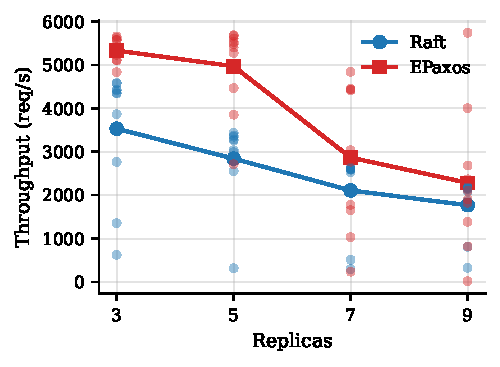
\includegraphics[width=0.85\columnwidth]{figures/throughput-scaling.pdf}
      \caption{Mean throughput by replica count at 100\,\% writes and
      concurrency 32. Points show individual repetitions.}
      \label{fig:throughput-scaling}
  \end{figure}

  Figure~\ref{fig:throughput-concurrency} shows the measured throughput
  across the concurrency sweep. Throughput increased with client concurrency
  for both protocols at every tested level. At concurrency 1, Raft recorded
  257\,req/s and EPaxos 174\,req/s. At concurrency 256, EPaxos recorded
  33{,}971\,req/s and Raft 17{,}845\,req/s. Across the sweep, the highest
  per-run value observed was 43{,}681\,req/s for EPaxos and 21{,}656\,req/s
  for Raft, both at concurrency 256. From concurrency 64 to 256, the Raft
  mean increased by a factor of 2.5 (7{,}020 to 17{,}845\,req/s) and the
  EPaxos mean by a factor of 3.2 (10{,}712 to 33{,}971\,req/s).

  \begin{figure}[t]
      \centering
      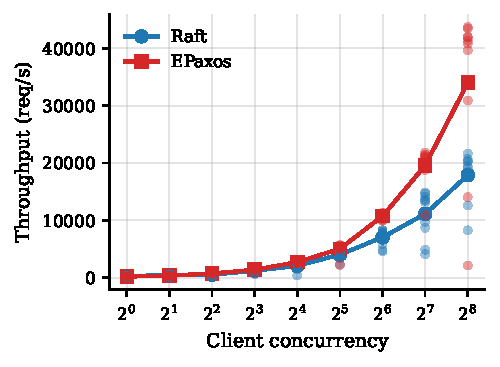
\includegraphics[width=0.85\columnwidth]{figures/throughput-concurrency.pdf}
      \caption{Mean throughput by client concurrency at 3 replicas and
      100\,\% writes. Points show individual repetitions.}
      \label{fig:throughput-concurrency}
  \end{figure}

  Figure~\ref{fig:throughput-write-ratio} shows the measured throughput
  across the write-ratio sweep at concurrency 32. Between 0\,\% and 100\,\%
  writes, the mean for EPaxos ranged from 4{,}926 to 5{,}332\,req/s and for
  Raft from 3{,}382 to 4{,}282\,req/s. Neither protocol showed a systematic
  trend across the write ratios tested: Raft's highest mean was at 100\,\%
  writes and its lowest at 90\,\%, while EPaxos's highest was at 10\,\% writes
  (8\% above its 100\,\% value).

  \begin{figure}[t]
      \centering
      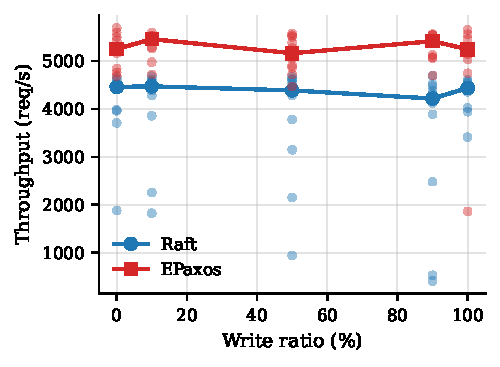
\includegraphics[width=0.85\columnwidth]{figures/throughput-write-ratio.pdf}
      \caption{Mean throughput by write ratio at 3 replicas and concurrency
      32. Points show individual repetitions.}
      \label{fig:throughput-write-ratio}
  \end{figure}

  Figure~\ref{fig:throughput-conflict-ratio} shows the measured throughput
  across the conflict-ratio sweep. Mean throughput ranged from 3{,}514 to
  4{,}425\,req/s for Raft and from 4{,}662 to 5{,}235\,req/s for EPaxos
  across conflict ratios of 0--100\,\%. The spread across repetitions within
  a configuration was of comparable magnitude to the spread across
  configurations in both cases.

  \begin{figure}[t]
      \centering
      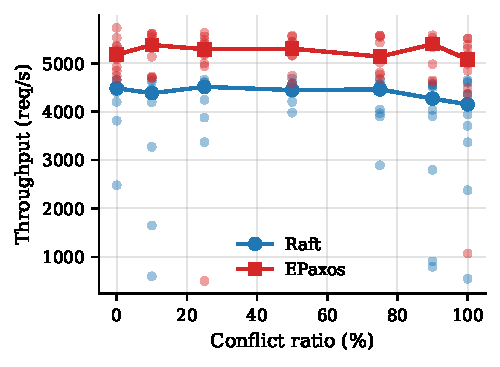
\includegraphics[width=0.85\columnwidth]{figures/throughput-conflict-ratio.pdf}
      \caption{Mean throughput by conflict ratio at 3 replicas, 100\,\%
      writes, and concurrency 32. Points show individual repetitions.}
      \label{fig:throughput-conflict-ratio}
  \end{figure}

  \subsection{Latency}

  Figure~\ref{fig:latency-replica-scaling} shows the measured median (p50)
  latency at each tested replica count. At the 3-replica baseline, the median
  was 12.3\,ms for Raft and 5.6\,ms for EPaxos. As replicas were added, the
  Raft median rose to 16.8\,ms at 5 replicas and 25.5\,ms at 7, then fell to
  22.8\,ms at 9, while the EPaxos median stayed between 5.6\,ms and 6.2\,ms
  across the same range (Table~\ref{tab:latency}).

  \begin{table}[t]
\caption{Median (p50) latency in milliseconds by replica count, at
100\,\% writes and concurrency 32.}
\label{tab:latency}
\begin{tabular}{lrr}
\toprule
Replicas & Raft p50 (ms) & EPaxos p50 (ms) \\
\midrule
3 & 12.3 & 5.6 \\
5 & 16.8 & 5.6 \\
7 & 25.5 & 6.0 \\
9 & 22.8 & 6.2 \\
\bottomrule
\end{tabular}
\end{table}


  \begin{figure}[t]
      \centering
      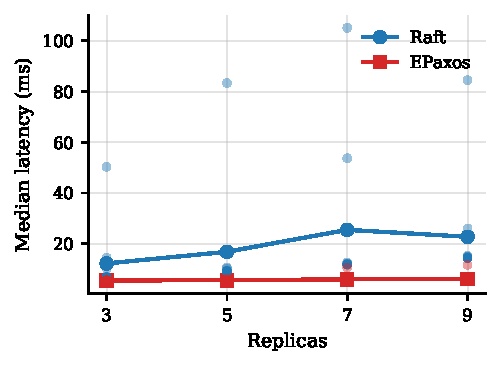
\includegraphics[width=0.85\columnwidth]{figures/latency-replica-scaling.pdf}
      \caption{Median (p50) latency by replica count at 100\,\% writes and
      concurrency 32. Points show individual repetitions.}
      \label{fig:latency-replica-scaling}
  \end{figure}

  Figure~\ref{fig:latency-concurrency} shows the measured median latency
  across the concurrency sweep. Median latency increased with concurrency for
  both protocols. At concurrency 1, the Raft median was 4.1\,ms and the
  EPaxos median 5.5\,ms; at concurrency 32, 7.4\,ms and 5.9\,ms; and at
  concurrency 256, 13.4\,ms and 14.0\,ms.

  \begin{figure}[t]
      \centering
      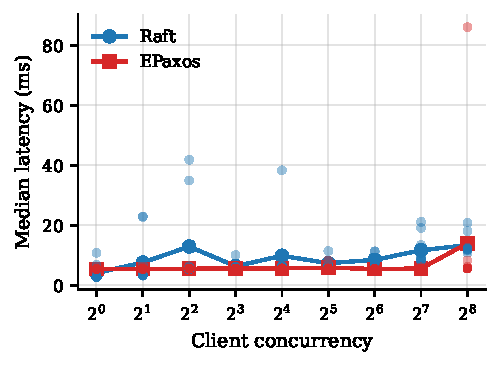
\includegraphics[width=0.85\columnwidth]{figures/latency-concurrency.pdf}
      \caption{Median (p50) latency by client concurrency at 3 replicas and
      100\,\% writes. Points show individual repetitions.}
      \label{fig:latency-concurrency}
  \end{figure}

  \subsection{Resource Utilisation}

  Figure~\ref{fig:resource-utilisation} summarises the per-replica resource
  measurements. Across all runs, mean per-replica CPU utilisation was 35.8\,\%
  for Raft and 35.0\,\% for EPaxos; mean peak per-replica RSS was 26.4\,MB
  for Raft and 46.8\,MB for EPaxos; and mean per-replica network rates were
  441\,kB/s RX and 443\,kB/s TX for Raft, and 408\,kB/s RX and 392\,kB/s
  TX for EPaxos.

  \begin{figure*}[t]
      \centering
      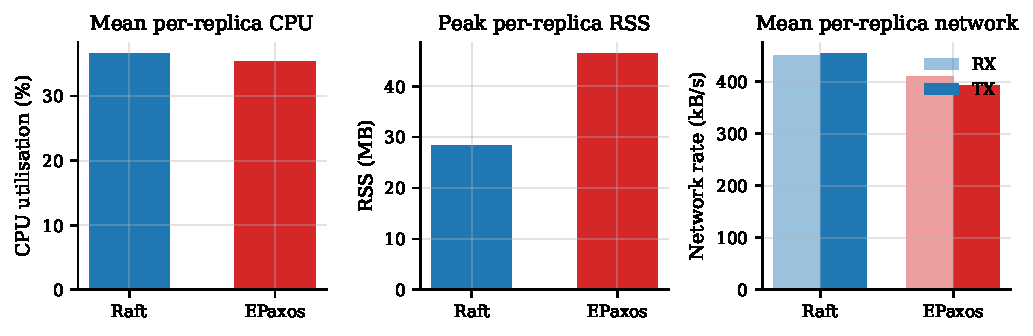
\includegraphics[width=0.85\textwidth]{figures/resource-utilisation.pdf}
      \caption{Mean per-replica CPU utilisation, peak per-replica RSS, and
      mean per-replica network rates, aggregated over all runs.}
      \label{fig:resource-utilisation}
  \end{figure*}

  Figure~\ref{fig:per-replica-cpu} shows the per-replica CPU utilisation in
  the 9-replica scaling runs. In the Raft runs, the per-replica means ranged
  from 16.3\,\% to 29.4\,\%: whichever replica held the leader role during a
  repetition used more CPU, and the leadership rotated across repetitions, so
  each replica's mean reflects the fraction of repetitions in which it led.
  In the corresponding EPaxos runs, the per-replica means ranged from
  22.4\,\% to 23.0\,\%, with no replica standing out.

  \begin{figure}[t]
      \centering
      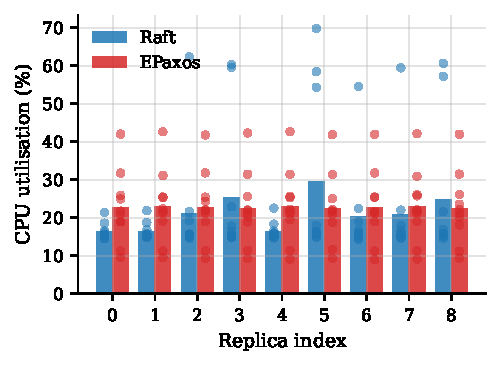
\includegraphics[width=0.85\columnwidth]{figures/per-replica-cpu.pdf}
      \caption{Per-replica CPU utilisation in the 9-replica scaling runs.
      Bars show the mean over repetitions; points show individual
      repetitions.}
      \label{fig:per-replica-cpu}
  \end{figure}

  \subsection{Failure Recovery Behaviour}

  Failure outcomes differed by failure type (Table~\ref{tab:failure},
  Figure~\ref{fig:failure-recovery}). Killing the Raft leader produced a
  write-availability gap of 1.81--4.74\,s and 2{,}169--4{,}133 failed
  requests. Killing a Raft follower produced a gap of 0.02--0.04\,s with no
  failed requests. Killing an EPaxos replica produced a gap of
  0.02--0.09\,s with 10--106 failed requests. All runs completed with status
  \texttt{success}; the failed requests are those issued during the
  transition.

  \begin{table}[t]
\caption{Failure behaviour at 3 replicas, 100\,\% writes, concurrency 32.
Gap is the largest interval with no successful write completion after
failure injection.}
\label{tab:failure}
\begin{tabular}{llrr}
\toprule
Failure & Protocol & Gap (s) & Failed req. \\
\midrule
Leader kill & Raft & 1.81--4.74 & 2{,}169--4{,}133 \\
Follower kill & Raft & 0.02--0.04 & 0 \\
Replica kill & EPaxos & 0.02--0.09 & 10--106 \\
\bottomrule
\end{tabular}
\end{table}


  \begin{figure*}[t]
      \centering
      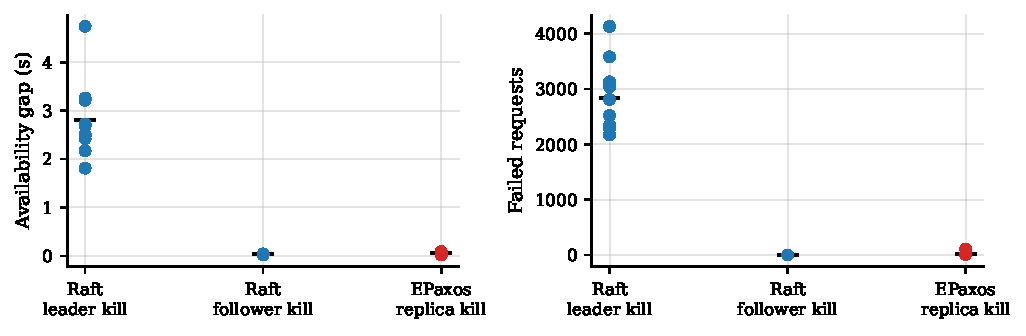
\includegraphics[width=0.80\textwidth]{figures/failure-recovery.pdf}
      \caption{Write-availability gap and failed requests by failure type at
      3 replicas, 100\,\% writes, concurrency 32. Points show individual
      repetitions; the bar marks the mean.}
      \label{fig:failure-recovery}
  \end{figure*}

  The election family, which isolates replicas to force repeated failed
  elections during a Raft leader failure, produced availability gaps that
  grow with the measured number of failed elections
  (Figure~\ref{fig:election-failure}, left): across the 60 measured runs the
  Pearson correlation between the measured failed elections (0--13) and the
  gap is $r=0.90$ ($p<10^{-4}$). This correlation is partly mechanical: the
  injection isolates the surviving replicas' transport for a duration
  proportional to the target, so a run with more failed elections has a
  longer gap by construction. To separate the injection duration from the
  recovery behaviour, the right panel shows the recovery time measured from
  the end of the isolation window to the first successful request. This
  decoupled metric is smaller and more variable but still increases with the
  measured election count ($r=0.41$, $p=0.001$, $n=60$): after the isolation
  expires, a cluster that experienced more failed elections takes longer to
  restore service, beyond the extra time the injection itself consumed.

  \begin{figure*}[t]
      \centering
      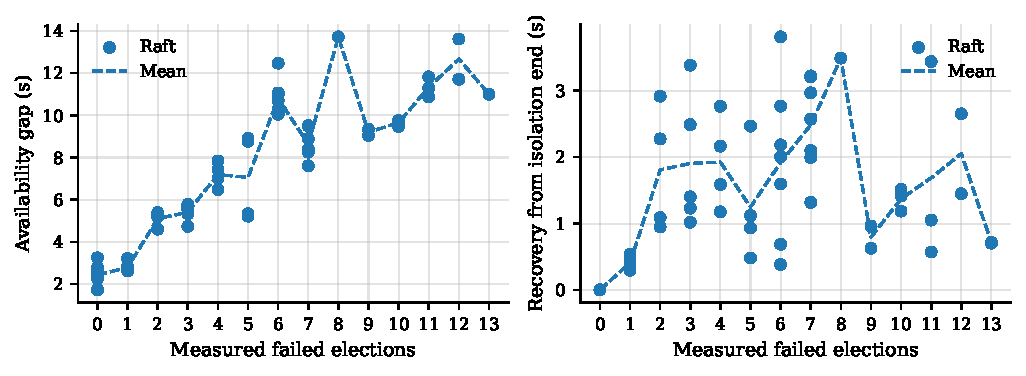
\includegraphics[width=0.85\textwidth]{figures/election-failure.pdf}
      \caption{Election-failure recovery in Raft at 3 replicas, 100\,\%
      writes, concurrency 32. Left: write-availability gap vs the measured
      number of failed elections (the gap includes the isolation duration,
      which is proportional to the target). Right: recovery time from the end
      of the isolation window to the first successful request, decoupled from
      the injection duration. Points show individual repetitions; the dashed
      line marks the mean per value.}
      \label{fig:election-failure}
  \end{figure*}

  \subsection{Correctness Validation}

  The measurements above assume that each implementation performs correct
  consensus execution. The correctness harness described in
  Section~\ref{sec:setup} verifies this independently of the performance
  benchmark. After each test the harness collects every replica's
  state-machine snapshot over the admin RPC and checks that (i) every
  replied request was applied exactly once, with no missing and no
  duplicate application; (ii) the surviving replicas' final states agree;
  (iii) after a restart, a restarted Raft replica's state matches the
  committed state, because Raft persists its log and every replica must
  catch up, while a restarted EPaxos replica is only required to be alive,
  because EPaxos keeps its state in memory; and (iv) new requests are
  processed after the fault.

  All 18 tests passed (Table~\ref{tab:correctness}): every replied request
  was applied exactly once on every replica, the surviving replicas agreed
  on the final state, the restarted Raft replicas recovered the committed
  state, and requests issued after each fault were processed normally. The
  per-test results are recorded in
  \texttt{lab/results/correctness/correctness.json}.

  \begin{table}[t]
\caption{Correctness-validation results: 2{,}000 deterministic requests per
test at 3 replicas, 100\,\% writes. Every replied request was applied exactly
once on every replica, surviving replicas agreed on the final state, and
requests issued after each fault were processed normally.}
\label{tab:correctness}
\small
\setlength{\tabcolsep}{4pt}
\begin{tabular}{@{}lllll@{}}
\toprule
Implementation & Sequential & c=8 & c=32 & Fault \\
\midrule
Raft (HashiCorp) & PASS & PASS & PASS & follower/leader \\
Raft (etcd)      & PASS & PASS & PASS & follower/leader \\
EPaxos (original) & PASS & PASS & PASS & replica \\
EPaxos (nvb)     & PASS & PASS & PASS & replica \\
\bottomrule
\end{tabular}
\end{table}

  \subsection{Communication Cost}

  The communication-cost family adds a fixed one-way latency (cost) to every
  inter-replica message, optionally with jitter, simulating a real network
  instead of the local loopback used by the other families. Figure
  \ref{fig:throughput-commcost} shows the measured mean throughput at each
  cost level (jitter 0) for the four implementations. The four
  implementations differ sharply in their sensitivity to added latency. The
  HashiCorp Raft implementation fell from 4{,}502\,req/s at cost 0 to
  1{,}280\,req/s at 10\,ms (a 72\,\% reduction), the most gradual decline of
  the four. The nvb EPaxos implementation fell from 4{,}346 to 833\,req/s
  (81\,\%), and the original EPaxos implementation from 5{,}527 to 221\,req/s
  (96\,\%). The etcd Raft implementation collapsed at the smallest tested
  cost: 6{,}420\,req/s at cost 0 fell to 375\,req/s at 1\,ms (94\,\%) and to
  45\,req/s at 10\,ms. The 95\,\% intervals of the means are separated
  between the implementations at every cost level above 0.

  \begin{figure}[t]
      \centering
      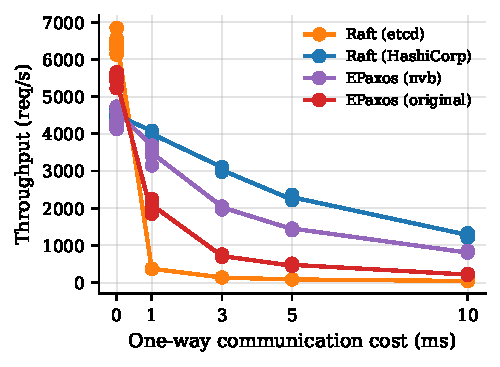
\includegraphics[width=0.85\columnwidth]{figures/throughput-commcost.pdf}
      \caption{Mean throughput by one-way communication cost at 3 replicas,
      100\,\% writes, and concurrency 32, for the four implementations.}
      \label{fig:throughput-commcost}
  \end{figure}

  The median latency grew correspondingly: at 10\,ms cost the p50 was
  22.6\,ms for HashiCorp Raft, 36.2\,ms for nvb EPaxos, 125.9\,ms for the
  original EPaxos, and 703.4\,ms for etcd Raft (Figure
  \ref{fig:latency-commcost}). The ordering of the implementations is the
  same for latency as for throughput, and the etcd Raft p50 at 10\,ms cost
  exceeds the 2{,}000\,ms request timeout only at the largest jitter levels.

  \begin{figure}[t]
      \centering
      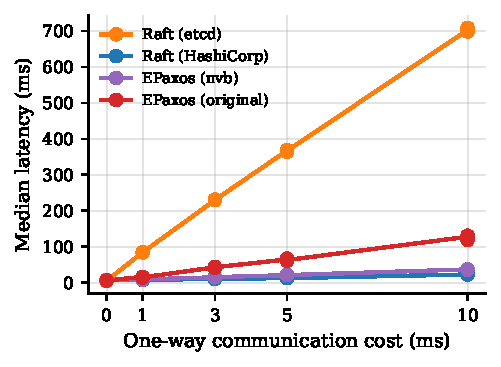
\includegraphics[width=0.85\columnwidth]{figures/latency-commcost.pdf}
      \caption{Median (p50) latency by one-way communication cost at 3
      replicas, 100\,\% writes, and concurrency 32, for the four
      implementations.}
      \label{fig:latency-commcost}
  \end{figure}

  Jitter had a much weaker effect than the cost itself. At the 5\,ms cost
  level, raising the jitter from 0\,\% to 100\,\% reduced throughput from
  2{,}316 to 1{,}760\,req/s for HashiCorp Raft (24\,\%), from 1{,}432 to
  1{,}082\,req/s for nvb EPaxos (24\,\%), from 479 to 305\,req/s for the
  original EPaxos (36\,\%), and from 87 to 59\,req/s for etcd Raft (32\,\%)
  (Figure \ref{fig:throughput-commcost-jitter}). The jitter adds at most
  $c \cdot j/100$ to each message, so at 100\,\% jitter the mean one-way
  delay rises from 5\,ms to 7.5\,ms; the measured throughput loss is
  consistent with that modest increase in mean delay rather than with the
  variance itself.

  \begin{figure}[t]
      \centering
      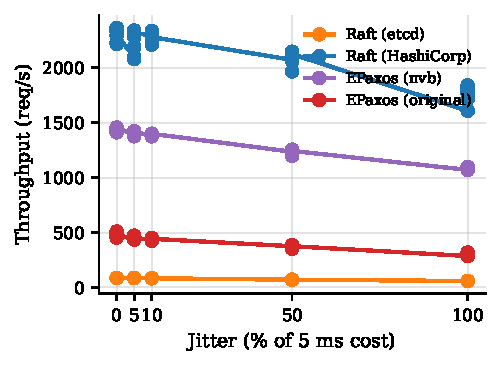
\includegraphics[width=0.85\columnwidth]{figures/throughput-commcost-jitter.pdf}
      \caption{Mean throughput by jitter at a 5\,ms one-way cost, 3 replicas,
      100\,\% writes, and concurrency 32, for the four implementations.}
      \label{fig:throughput-commcost-jitter}
  \end{figure}

  \subsection{Summary of Findings}

  The measurements support the following observations under the conditions
  tested:

  \begin{itemize}
  \item At each tested replica count, the measured mean throughput for EPaxos
    was higher than that for Raft, with the largest relative difference at 5
    replicas (1.75$\times$); the 95\,\% intervals are separated at 3 and 5
    replicas but overlap at 7 and 9.
  \item Throughput decreased with replica count for both protocols; from 3 to
    9 replicas the mean decreased by 57\% for EPaxos and 50\% for Raft.
  \item At concurrency 256, the measured mean throughput was 33{,}971\,req/s
    for EPaxos and 17{,}845\,req/s for Raft; the highest per-run values
    observed were 43{,}681\,req/s and 21{,}656\,req/s respectively.
  \item Median latency was lower for EPaxos at every tested replica count,
    and increased with replica count only for Raft.
  \item In the 9-replica runs, per-replica CPU means ranged from 16.3\,\% to
    29.4\,\% in Raft, where leadership rotated between repetitions, and from
    22.4\,\% to 23.0\,\% in EPaxos, where no replica stood out.
  \item Write ratio and conflict ratio produced no systematic throughput
    trend in either protocol over the ranges tested.
  \item Raft leader-kill experiments recorded write-availability gaps of
    1.81--4.74\,s and 2{,}169--4{,}133 failed requests, while follower-kill
    and EPaxos replica-kill experiments recorded gaps under 0.1\,s with at
    most 106 failed requests.
  \item The measured failed-election count (0--13, never the configured
    target) predicts the availability gap almost linearly ($r=0.90$,
    $n=60$), and remains a significant predictor of the decoupled
    post-isolation recovery time ($r=0.41$, $p=0.001$).
  \item Under added one-way communication cost, the four implementations
    differed sharply in sensitivity: HashiCorp Raft lost 72\,\% of its
    throughput at 10\,ms cost, nvb EPaxos 81\,\%, the original EPaxos
    96\,\%, and etcd Raft collapsed by 94\,\% at 1\,ms already. Jitter at a
    5\,ms cost reduced throughput by 24--36\,\% at 100\,\% jitter, a much
    weaker effect than the cost itself.
  \end{itemize}